\documentclass[11pt]{article}
\usepackage[margin = 1in]{geometry}
\usepackage{amsmath}
\usepackage{amssymb}
\usepackage{amsthm} % for proof environment
\usepackage{enumitem}
\usepackage{graphicx}
\usepackage{indentfirst}
\usepackage{caption}
\usepackage{lscape}
\usepackage{multirow}
\usepackage{array}
\usepackage{setspace}
\setlist{nolistsep}
\usepackage[round]{natbib}
\usepackage{accents}
\usepackage{caption}
\usepackage{subcaption}

\newcommand{\ubar}[1]{\underaccent{\bar}{#1}}
\newcommand{\p}{\prime}
\newcommand{\ev}{\mathbb{E}}
\newcommand{\lagr}{\mathcal{L}}
\newcommand{\inv}[1]{#1^{-1}}
\newcommand{\R}{{\rm I\!R}}
\newcommand{\U}{\mathcal{U}}
\renewcommand{\H}{\mathcal{H}}
\newcommand{\pderiv}[2]{\frac{\partial#1}{\partial #2}}

\begin{document}
    \begin{flushleft}
        Optimal Taxation with Heterogeneous Rates of Return \\
        Progress: \today
    \end{flushleft}

\section{Introduction}
The primary goal of this paper is to characterize optimal taxes in a model with heterogeneous rates of return. To this end, we draw on two strains in the literature. The first is the New Dynamic Public Finance (NDPF) literature, as reviewed in \cite{golosov2006new} and \cite{kocherlakota2010new}, which extends the optimal taxation framework of \cite{mirrlees1971exploration} into dynamic and stochastic settings. Additionally, we draw on literature which has attempted to match empirical measures of the distribution of wealth in heterogeneous-agent models. In particular, we consider optimal taxation in a model similar to that of \cite{benhabib2011distribution}, wherein the wealth distribution displays a Pareto tail, the mass of which is determined by capital, rather than labor, income risk. 

\section{Model}
\subsection{Households}
Thus far, I have restricted attention to simple two-period versions of the model. The economy is populated by a continuum of households of measure one. Each household has type \( \theta\in\Theta \) and initial wealth \( w_0 \). I assume that the distribution of \( \theta \) has PDF \( f(\theta) \) and CDF \( F(\theta) \). In the first period, the household allocates consumption between consumption and savings. If a household saves \( k \), they are able to produce output in the second period according to the production function \( y = \theta k \). Households discount the future at rate \( \beta \), and derive utility from consumption according to the twice continuously differentiable function \( u(c) \). With this setup, the model is similar to the static model of \cite{mirrlees1971exploration}: households face a tradeoff between current and future consumption, rather than consumption and leisure. 

\subsection{Government}
I assume that the government cannot observe type \( \theta \) or investment \( k \) separately; it can only observe and thus levy a tax on output, denoted \( T(\theta k) \). The government's objective is to maximize total utility
\begin{equation}
    \int_\Theta \U(\theta)f(\theta)d\theta \label{obj_tax}
\end{equation}
where \( \U(\theta) \) is total two-period utility of type \( \theta \):
\begin{equation}
    \U(\theta) = \max_{0\leq k \leq w_0} u(w_0 - k) + \beta u(\theta k - T(\theta k)) \label{bigu_tax}
\end{equation}
I require that for each type, \( 0 \leq k(\theta) \leq w_0 \), and that no taxes are levied in the first period, thus ensuring that the resource constraint holds trivially in the first period. The resource constraint faced by the government in the second period, then, is 
\begin{equation}
    \int_\Theta T(\theta k(\theta))f(\theta)d\theta \geq E \label{rc_tax}
\end{equation}
where \( E \) denotes government expenditures. 

Additionally, the government faces incentive compatibility constraints, which require that the tax function \( T(\cdot) \) be such that no type \( \theta \) is better off imitating type \( \hat{\theta} \). Formally, these constraints require that the consumer's saving and consumption decisions be at an optimum. The first-order condition of (\ref{bigu_tax}) for \( k \) gives
\begin{equation}
    u^\p(w_0 - k) = \beta \theta (1 - T^\p)u^\p (\theta k - T(\theta k)) \label{foc_hh_tax}
\end{equation}
The envelope condition for (\ref{bigu_tax}), meanwhile, gives 
\begin{equation}
    \U^\p(\theta) = \beta k u^\p (\theta k - T(\theta k)) (1 - T^\p) \label{env_hh_tax}
\end{equation}
Combining (\ref{foc_hh_tax}) and (\ref{env_hh_tax}) gives the law of motion for \( \U \):
\begin{equation}
    \U^\p(\theta) = \frac{u^\p(w_0 - k)k}{\theta} \label{lom_tax}
\end{equation}
Thus, the government's problem is to maximize (\ref{obj_tax}), subject to (\ref{bigu_tax}), (\ref{rc_tax}), and (\ref{lom_tax}). 

As noted by \cite{mirrlees1971exploration}, the government's problem can be equivalently characterized as a mechanism design problem. Denote consumption in the second period as \( c(\theta) = \theta k\theta - T(\theta k(\theta)) \). In this formulation, the government collects reports from households on their type \( \theta \), and allocates to them first-period output \( y(\theta) \) and second-period consumption \( c(\theta) \). The government's objective, again, is to maximize total utility (\ref{obj_tax}), where now 
\begin{equation}
    \U(\theta) = u\left( w_0 - \frac{y(\theta)}{\theta} \right) + \beta u(c(\theta))) \label{bigu_md}
\end{equation}
The envelope condition for (\ref{bigu_md}) gives 
\begin{align}
    \U^\p(\theta) &= u^\p\left( w_0 - \frac{y(\theta)}{\theta} \right)\frac{y(\theta)}{\theta^2} \notag \\
    &= u^\p(w_0 - k)\frac{k}{\theta} 
\end{align}
exactly as in (\ref{lom_tax}). The resource constraint (\ref{rc_tax}) can be rewritten as 
\begin{equation}
    \int_\Theta \left[ \theta k(\theta) - c(\theta) \right]f(\theta) d\theta \geq E \label{rc_md}
\end{equation}
The incentive constraint again require that agents behave according to their prescribed type, or formally,
\begin{equation}
    \theta \in \arg\max_{\hat{\theta}} u\left( w_0 - \frac{\hat{\theta} k}{\theta} \right) + \beta u(c_1(\hat{\theta}))\quad \forall \theta\in\Theta \label{ic_md}
\end{equation}
The constraints in (\ref{ic_md}) can be interpreted as follows: the planner collects reports \( \hat{\theta} \), and allocates output \( y(\hat{\theta}) \) and consumption \( c(\hat{\theta}) \). Thus, if an agent of type \( \theta \) claims to be of type \( \hat{\theta} \), she will receive \( c(\hat{\theta}) \), but in return, she will be required to produce output \( y(\hat{\theta}) \), requiring investment \( \frac{\hat{\theta}k}{\theta} \). 

\section{Continuous-Type Case}

In this section, I consider the case where \( \Theta = [\ubar{\theta}, \bar{\theta}] \) is continuous. 

\subsection{Frisch Elasticity of Capital Supply}
In order to characterize the optimal tax schedule, I derive the Frisch Elasticity of capital supply \( \varepsilon_k^\lambda \). Intuitively, \( \varepsilon_k^\lambda \) measures the elasticity of \( k \) with respect to the marginal post-tax return, holding marginal utility of consumption in the \textit{second} period constant. Following \cite{paradisi_notes}, I begin with the household's problem:
\begin{align}
    \max_{c,k}\quad U(k, c) &= u(w - k) + \beta u(c) \\
    \text{s.t.}\quad c &= \theta k - T(\theta k) \label{hh_bc}
\end{align}
Where \( T(\cdot) \) is the tax. Let \( \phi = \theta(1 - T^\p) \) denote the marginal return, net of tax. The fist-order conditions for the household's problem are 
\begin{align}
    U_c &= \beta u^\p(c) = \lambda \label{e_foc_1} \\
    U_k &= -u^\p(w - k) = -\phi \lambda \label{e_foc_2}
\end{align}
where \( \lambda \) is the multiplier on (\ref{hh_bc}), which will be held constant in this derivation. Totally differentiating (\ref{e_foc_1}) and (\ref{e_foc_2}) gives the following set of two equations in two unknowns:
\begin{equation}
    \begin{bmatrix}
        U_{cc} & U_{ck} \\
        U_{ck} & U_{kk}
    \end{bmatrix} \begin{bmatrix}
        \frac{dc}{d\phi} \\ \frac{dk}{d\phi} 
    \end{bmatrix} = \begin{bmatrix}
        0 \\ -\lambda
    \end{bmatrix}
\end{equation}
Solving by inverting gives 
\begin{align}
    \frac{dk}{d\phi} &= -\frac{U_{cc}\lambda}{U_{cc}U_{kk} - U_{ck}^2} \notag \\
    &= -\frac{U_{cc}\frac{U_k}{\phi}}{U_{cc}U{kk} - U_{ck}^2} \\
    &= -\frac{U_k}{\phi\left( U_{kk} - \frac{U_{ck}^2}{U_{cc}} \right)}
\end{align}
where the second equality follows from (\ref{e_foc_2}). Note also that in this formulation, \( U_{ck} = 0 \). Thus, the elasticity is given by 
\begin{equation}
    \varepsilon_k^\lambda = \frac{dk}{d\phi} \frac{\phi}{k} = -\frac{u^\p(w - k)}{ku^{\p\p}(w - k)} \label{frisch}
\end{equation}
\subsection{Optimal Tax Problem}
The problem faced by the social planner is as follows: 
\begin{align*}
    \max_{c(\theta), k(\theta)} &\int_{\ubar{\theta}}^{\bar{\theta}} \U(\theta)f(\theta)d\theta \\
    &\text{s.t.} \\
    \U(\theta) &= u(w - k(\theta)) + \beta u(c(\theta)) \\
    \U^\p(\theta) &= u^\p(w - k(\theta))\frac{k(\theta)}{\theta} \\
    \int_{\ubar{\theta}}^{\bar{\theta}} &\left[ \theta k(\theta) - c(\theta) \right] f(\theta)d\theta \ge E
\end{align*}
The Lagrangean (after integrating by parts) for the above problem is 
\begin{multline}
    \lagr = \int_{\ubar{\theta}}^{\bar{\theta}} \U(\theta)f(\theta)d\theta + \int_{\ubar{\theta}}^{\bar{\theta}} \gamma(\theta)\left[ u(w - k) + \beta u(c) - \U(\theta) \right]d\theta + \\ \int_{\ubar{\theta}}^{\bar{\theta}} u^\p(w - k)\frac{k}{\theta}\mu(\theta)d\theta + \U(\theta)\mu\theta\Big|_{\ubar{\theta}}^{\bar{\theta}} - \int_{\ubar{\theta}}^{\bar{\theta}}\U(\theta)\mu^\p(\theta)d\theta + \\ \lambda\left( \int_{\ubar{\theta}}^{\bar{\theta}}\left[ \theta k - c \right]f(\theta)d\theta - E \right) \label{plan_lag}
\end{multline}
The first-order conditions give the following equalities:
\begin{align}
    \mu^\p(\theta) &= \gamma(\theta) - f(\theta) \label{foc_U} \\
    \mu(\ubar{\theta}) &= \mu(\bar{\theta}) = 0 \label{foc_mu_bar} \\
    \gamma(\theta)u^\p(w - k) &= \lambda\theta f(\theta) + \frac{\mu(\theta)}{\theta}\left[ u^\p(w - k) - ku^{\p\p}(w - k) \right] \label{foc_k} \\
    \gamma(\theta) &= \frac{\lambda f(\theta)}{\beta u^\p(c)} \label{foc_c}
\end{align}
Letting \( \tau(\theta) = T^\p(\theta k(\theta)) \), the individual optimality condition gives 
\begin{equation}
    1 - \tau = \frac{u^\p(w - k)}{\beta \theta u^\p(c)} \label{ind_opt}
\end{equation}
Thus, using (\ref{foc_c}), 
\begin{align*}
    \lambda \theta f(\theta) - \gamma(\theta)u^\p(w - k) &= -\frac{u^\p(w - k)\lambda\theta f(\theta)}{\beta u^\p(c)} + \lambda\theta f(\theta) \\
    &= \lambda\theta f(\theta)\tau
\end{align*}
Substituting the second equality above into (\ref{foc_k}) gives 
\begin{align}
    \lambda\theta f(\theta)\tau &= -\frac{\mu(\theta)}{\theta}\left[ u^\p(w - k) - ku^{\p\p}(w - k) \right] \notag \\
    &= \frac{\mu(\theta)}{\theta} u^\p(w - k)\left( \frac{1}{\varepsilon_k^\lambda} + 1 \right) \notag \\
    &= \mu(\theta)\frac{\beta u^\p(c)}{1 - \tau} \left( \frac{1}{\varepsilon_k^\lambda} + 1 \right) \label{tax_eps}
\end{align}
where the second equality follows from the definition of elasticity in (\ref{frisch}) and the third from the individual optimality condition in (\ref{ind_opt}). Finally, integrating (\ref{foc_U}) and using the boundary condition at \( \bar{\theta} \) in (\ref{foc_mu_bar}) gives the following expression for \( \mu(\theta) \):
\begin{align}
    \mu(\theta) &= \int_{\theta}^{\bar{\theta}} \left[ \gamma(t) - f(t) \right]dt \notag \\ 
    &= \int_{\theta}^{\bar{\theta}} f(\theta)\left( \frac{\lambda}{\beta u^\p(c)} - 1 \right)d\theta \label{mu_exp}
\end{align}
Combining (\ref{tax_eps}) and (\ref{mu_exp}) gives the first-order condition for the optimal tax on capital income:
\begin{equation}
    \frac{\tau}{1 - \tau} = \left( \int_{\theta}^{\bar{\theta}} f(\theta)\left( \frac{\lambda}{\beta u^\p(c)} - 1 \right)d\theta \right)\left(\frac{\beta u^\p(c(\theta))}{\lambda \theta f(\theta)}\right)\left( \frac{1}{\varepsilon_k^\lambda} + 1 \right) \label{tax_foc}
\end{equation}
This condition is similar to the ``ABC'' condition in \cite{diamond1998optimal}: the three terms in (\ref{tax_foc}) show that the optimal tax depends on redistributive motives, the distribution \( f(\theta) \), and elasticity, respectively. 

\section{Two-Type Case}

This section presents some computational results on a simple version of the model, in order to get a sense of what the optimal allocations are. In sections \ref{t2_imm} and \ref{t2_mob}, I present the results from using Matlab to solve the planner's problem, subject to the resource and incentive constraints. 

\subsection{Immobile Capital} \label{t2_imm}
Here, I consider a model in which households are one of two types \( \theta\in\{\theta_L, \theta_h\} \) with \( \Pr(\theta = \theta_H) = \pi \). The social planner solves the usual problem:
\begin{align}
    \max &\sum_{i \in\{L,H\}}\left[ u(w - k(\theta_i)) + \beta u(c(\theta)) \right]\pi_i \\ 
    &\text{s.t.} \notag \\
    &\sum_{i \in\{L,H\}}\left[ \theta_i k(\theta_i) - c(\theta_i) \right]\pi_i \ge E \\
    &u(w - k(\theta_H)) + \beta u(c(\theta_H)) \ge u\left( w - \frac{\theta_L}{\theta_H}k(\theta_L) \right) + \beta u(c(\theta_L)) \label{ic_H} \\
    &u(w - k(\theta_L)) + \beta u(c(\theta_L)) \ge u\left( w - \frac{\theta_H}{\theta_L}k(\theta_H) \right) + \beta u(c(\theta_H)) 
\end{align}

I assume that \( u(c) = \log(c) \), and use the following parametrization:
\begin{align*}
    \beta &= 0.95 & w &= 1.2 \\
    E &= 0 & \pi &= 0.3 
\end{align*}

In general, the planner requires that households of type \( \theta_L \) invest in the first period. This level of investment can be low, particularly if \( \theta_H \) is large in relation to \( \theta_L \). However, it does seem that for most specifications, the planner finds it optimal to have \( k(\theta_L) > 0 \), likely in part to satisfy the incentive constraint for the high type (\ref{ic_H}). Figure \ref{fig_imm} shows the optimal allocations for the high and low types across different values of the ratio \( \theta_H / \theta_L \), for \( \theta_L = 1.02 \). 
%
\begin{figure}[!ht]
    \centering
    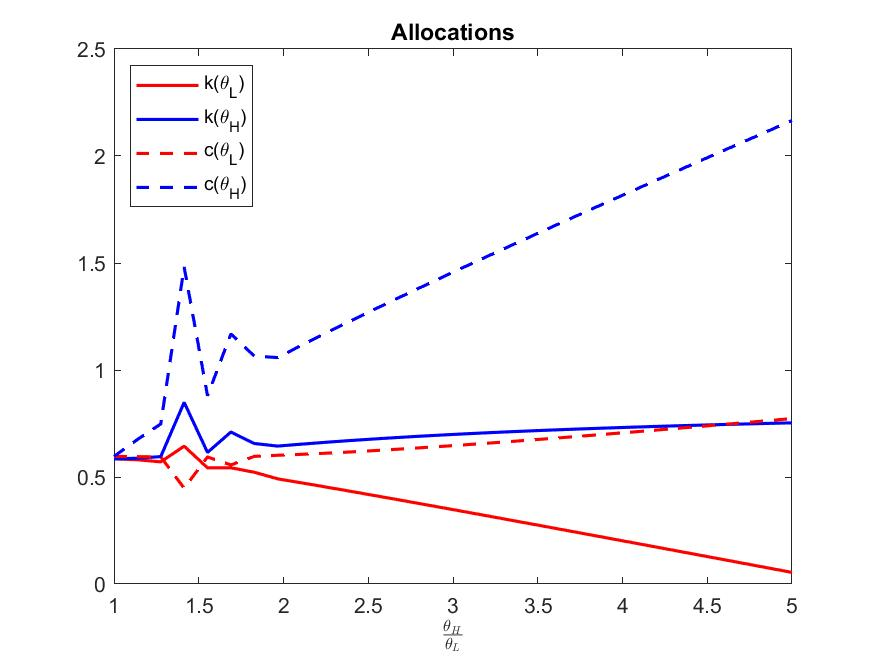
\includegraphics[scale = 0.5]{figures/immob.jpg}
    \caption{Optimal Allocations}
    \label{fig_imm}
\end{figure}

\subsection{Mobile Capital} \label{t2_mob}

Here I consider the same model as in section \ref{t2_imm}, but allow for the borrowing and lending of risk-free bonds \( b \) between the households in the first period. Thus, the planner's problem becomes

\begin{align}
    \max &\sum_{i \in\{L,H\}}\left[ u(w - k(\theta_i) - b(\theta_i)) + \beta u(c(\theta)) \right]\pi_i \\ 
    &\text{s.t.} \notag \\
    &\sum_{i \in\{L,H\}}\left[ \theta_i k(\theta_i) - c(\theta_i) \right]\pi_i \ge E \\
    &\sum_{i \in\{L,H\}}b(\theta_i)\pi_i = 0 \\ 
    &u(w - k(\theta_H) - b(\theta_H)) + \beta u(c(\theta_H)) \ge u\left( w - \frac{\theta_L}{\theta_H}k(\theta_L) - b(\theta_L)\right) + \beta u(c(\theta_L)) \label{ic1_mob} \\
    &u(w - k(\theta_L) - b(\theta_L)) + \beta u(c(\theta_L)) \ge u\left( w - \frac{\theta_H}{\theta_L}k(\theta_H) - b(\theta_H) \right) + \beta u(c(\theta_H)) \label{ic2_mob}  
\end{align}

Aside from the allowance for borrowing and lending, the model is the same as in section \ref{t2_imm}. In this case, if \( \theta_H \) is sufficiently large relative to \( \theta_L \), then \( k(\theta_L) = 0 \). The optimal borrowing and lending allocations call for \( \theta_H \) types to be net borrowers in the first period, allowing them to invest more, and for \( \theta_L \) types to be net lenders. Figure \ref{fig_mob} shows the optimal allocations for each type. 

\begin{figure}[!ht]
    \centering
    \begin{subfigure}{0.49\textwidth}
        \centering
        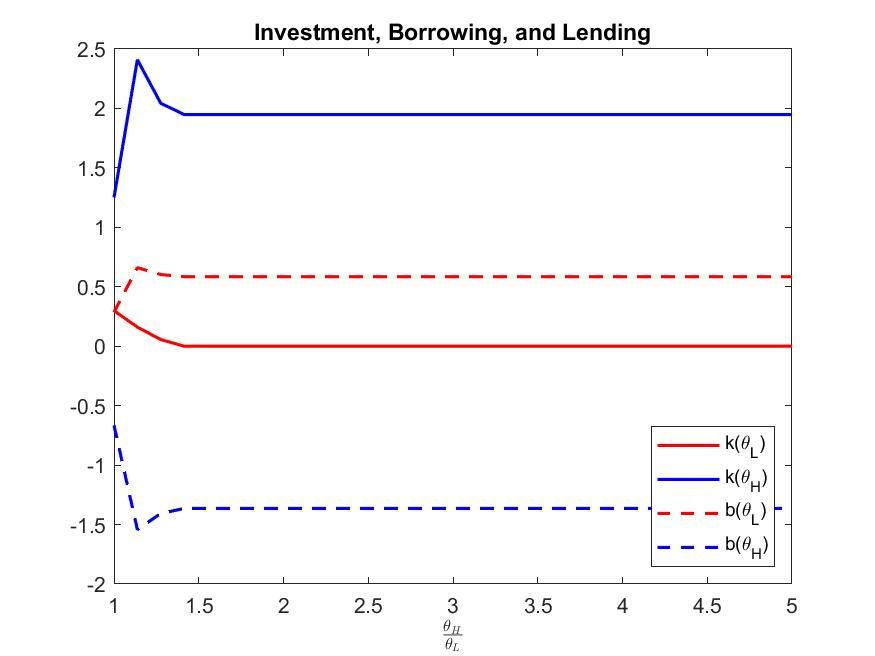
\includegraphics[scale = 0.3]{figures/inv_mob.jpg}
    \end{subfigure}
    \hfill
    \begin{subfigure}{0.49\textwidth}
        \centering
        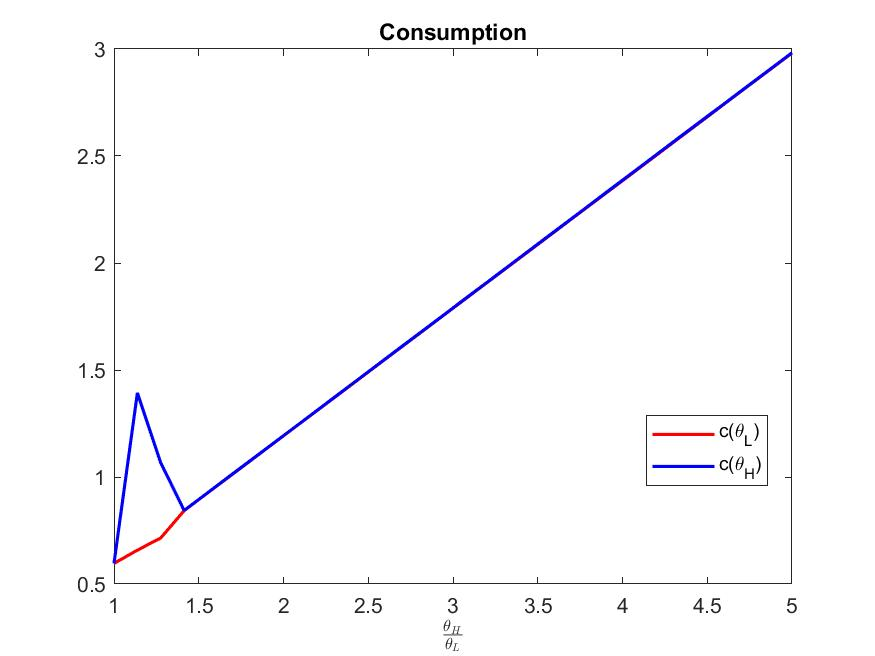
\includegraphics[scale = 0.3]{figures/cons_mob.jpg}
    \end{subfigure}
    \caption{Optimal Allocations with Mobile Capital}
    \label{fig_mob}
\end{figure}

The right-hand panel of Figure \ref{fig_mob} shows that with the exception of one \( (\theta_L, \theta_H) \) pair, consumption is equated between the two types. While this would seem to violate the incentive constraints (\ref{ic1_mob}) and (\ref{ic2_mob}), note that this is the consumption in the \textit{second} period. Where the consumption values differ is in the first period, which both types value more. 

\section{Next Steps}
\subsection{Extension to Dynamic Stochastic Settings}
My next step is to extend this deterministic, static model into a fully dynamic and stochastic setting. I plan to extend the model to make the agents infinitely lived, and produce according to the production function \( y = \theta k \varepsilon \), where \( \varepsilon \) is an idiosyncratic shock, the distribution of which depends on \( \theta \). As originally shown in \cite{golosov2003optimal}, the uncertainty in next-period output can give rise to nonnegative capital taxation. 

\bibliographystyle{named}
\bibliography{summer_paper}
\end{document}